\subsection{The interaction Lagrangian.}
\subsection{The brain as the principal receiver.}
\subsection{The heart as a modulator.}
\subsection{The complementary relation.}

\subsection{Measuring \texorpdfstring{$\Phi$}{Phi}: cortex versus cerebellum}
Postulate 2 states that it is the geometry of the network, not the number of neurons, that determines reception. To make the claim numerically checkable I implemented a tractable proxy for $\Phi$: the Kullback--Leibler divergence between the full model and the model in which the links across a cut are removed, minimised over all bipartitions, on Glauber dynamics. It is not the exact $\Phi$ of IIT 3.0; it is an approximation with the same ordinal signature.

\begin{table}[H]
\centering
\begin{tabular}{@{}cccc@{}}
\toprule
Units & $\Phi$ cortex & $\Phi$ cerebellum & Ratio \\ \midrule
4 & $0.243 \pm 0.063$ & $0.012 \pm 0.014$ & 20.6 \\
6 & $0.259 \pm 0.049$ & $0.045 \pm 0.015$ & 5.8 \\
8 & $0.245 \pm 0.042$ & $0.036 \pm 0.030$ & 6.9 \\ \bottomrule
\end{tabular}
\caption{$\Phi$ for recurrent and feedforward networks, averaged over four random networks for each size.}
\label{tab:phi}
\end{table}

The recurrent network integrates 2--20 times more than the feedforward one for the same number of units. The qualitative conclusion of version 30 is therefore supported numerically, within the limits of the proxy.

\begin{figure}[H]
\centering
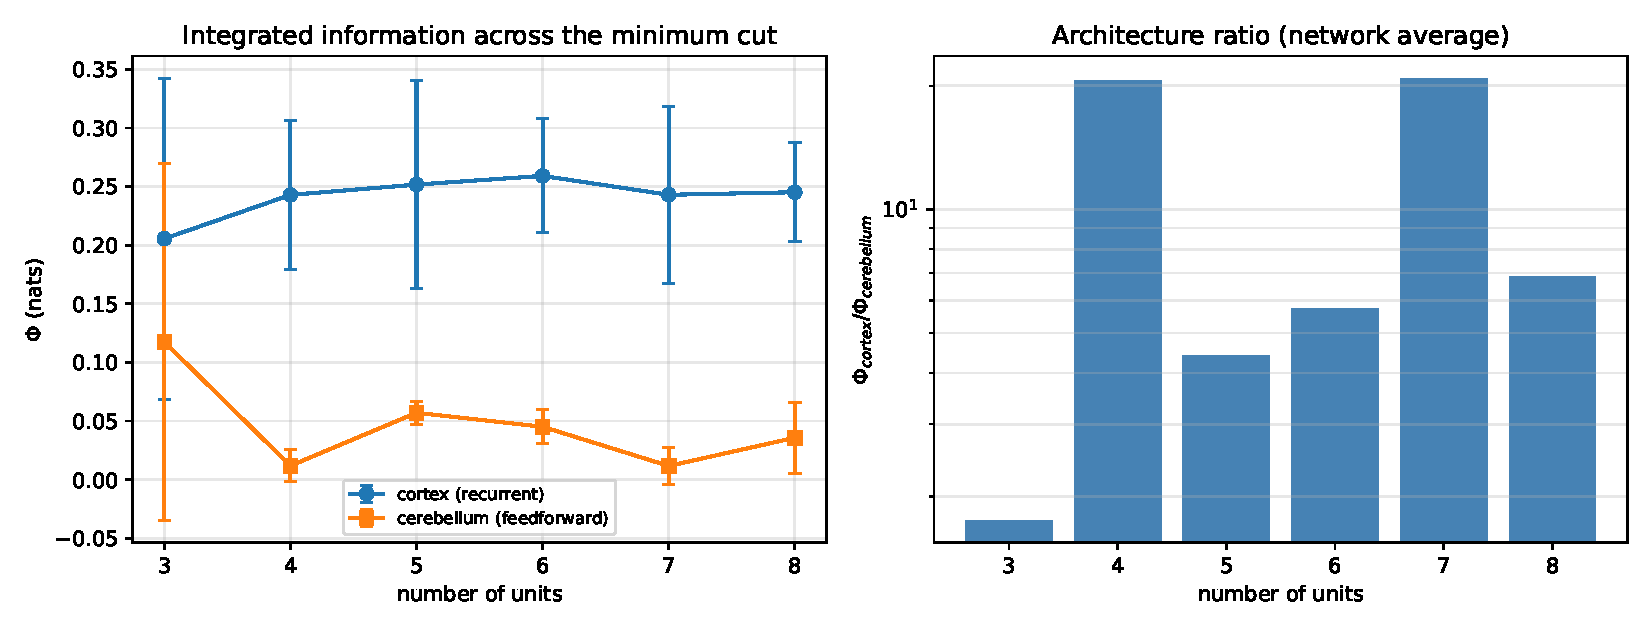
\includegraphics[width=0.9\textwidth]{figures/fig03_phi_architecture.pdf}
\caption{$\Phi$ for the two architectures, with the standard deviation over four random networks, and the ratio between them.}
\label{fig:phi}
\end{figure}

\section{Derivation of the Yukawa Coupling}
\subsection{The mechanism.}
\subsection{The estimate (expanded):} The general formula is $g_A \sim (M_4/M_{12})^5$. To obtain a numerical value we assume that the compactification scale is $M_{12} \sim 10^{19}$ GeV (the Planck scale) and that the electroweak scale is $M_4 \sim 10^3$ GeV. Then:
\begin{equation}
g_A \sim \left(\frac{10^3}{10^{19}}\right)^5 = (10^{-16})^5 = 10^{-80}
\end{equation}
This value is extremely small, which means that the coupling is very weak. It is important to stress that the overlap factors between the wave functions of the KK modes and the branes cannot raise the effective value to $\sim 10^{-3}$: the overlap of normalised wave functions is at most 1, so a factor of $10^{77}$ would be required, which is impossible. The value adopted in this paper is therefore $g_A \sim 10^{-80}$.

This value is also the only one compatible with the data. If the field coupled Yukawa-wise to nucleons, the force relative to gravity would be
\begin{equation}
\alpha = \frac{g_A^2\, \hbar c}{G\, m_p^2} = g_A^2 \times 1.69\times10^{38}.
\end{equation}
For $g = 10^{-3}$ this would give $\alpha \approx 1.7\times10^{32}$, excluded by laboratory tests by roughly 35 orders of magnitude. The 7\% constraint quoted in the introduction implies $g < 2\times10^{-20}$. Moreover, a coupling $g = 10^{-3}$ would give the mode a lifetime of order $10^{-3}$ s, incompatible with the stability of dark matter. The estimate $g_A \sim 10^{-80}$ is therefore what makes the theory predictive rather than merely consistent.
\subsection{Debye screening.}
\subsection{The effective force.}

\section{Tachyons as Intermediaries}
\subsection{The tachyonic spectrum:} $m_n^2 = n^2/R^2 - \mu_A^2$.
\subsection{The tachyonic coupling.}
\subsection{The bradyon--tachyon relation.}
\subsection{What the tachyons carry.}

\section{The Vacua of the Akashic Field}
\subsection{What is a vacuum?}
\subsection{The three types of vacuum.}
\subsection{The vacuum of the akashic field.}
\subsection{Multiple vacua.}

\section{Wave--Particle Duality}
\subsection{The mechanism in four steps.}
\subsection{What the wave carries.}
\subsection{The tree analogy.}

\section{The Complete Equations of Motion}
\subsection{The akashic equation.}
\subsection{The consciousness equation.}
\subsection{The equation of the exotic bosons.}
\subsection{The 12D Einstein equation.}

\newpage
